\subsection{Overview}
We need to design a system in which the user asks to the system to store an appointment and calculate the best path from a starting location to the appointment location. \\
Since this interaction between user and system can be summarize as:
\begin{enumerate}
	\item User request a service to the system.
	\item System responds to the user with the requested service.
\end{enumerate}
Based on this, we decide to use a client-server architectural approach.
\begin{figure}[H]
	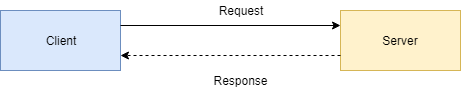
\includegraphics{Img/ClientServerArchitecture}
	\caption{Client Server architecture}
	\label{fig:clientserver}
\end{figure}
Furthermore, the system can be divided into three different subsystems: the presentation layer, the application layer and the data layer as we can see in \autoref{fig:overview}. 
\begin{itemize}
	\item The \emph{Presentation Layer} provides the GUI of the system. This layer contains
	the mobile application and the web pages.
	\item The \emph{Application Layer} contains the logic of the application,that receives 		the requests from the user, computes the best path to reach the appointment, checks the 	weather and the road conditions and executes the dynamic web pages of the web site.
	\item The \emph{Data Layer} stores and maintains the data needed from the system to 		works properly, i.e. user’s information and user’s appointment information.
\end{itemize}
\begin{figure}
	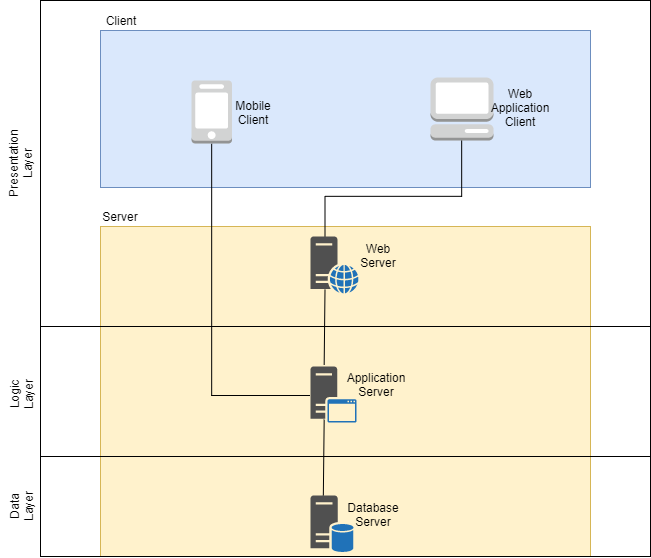
\includegraphics[width=\textwidth, height=\textheight, keepaspectratio=true]{Img/Overview}
	\caption{Overview of the system architecture}
	\label{fig:overview}
\end{figure}




\clearpage
\subsection{Component View}

\clearpage
\subsection{Deployment View}

\clearpage
\subsection{Runtime View}

\clearpage
\subsection{Component Interfaces}

\clearpage
\subsection{Selected architectural styles and patterns}

\clearpage
\subsection{Other design decision}